\begin{figure}[ht]
    \centering
    %\begin{adjustbox}{width=0.8\linewidth}
        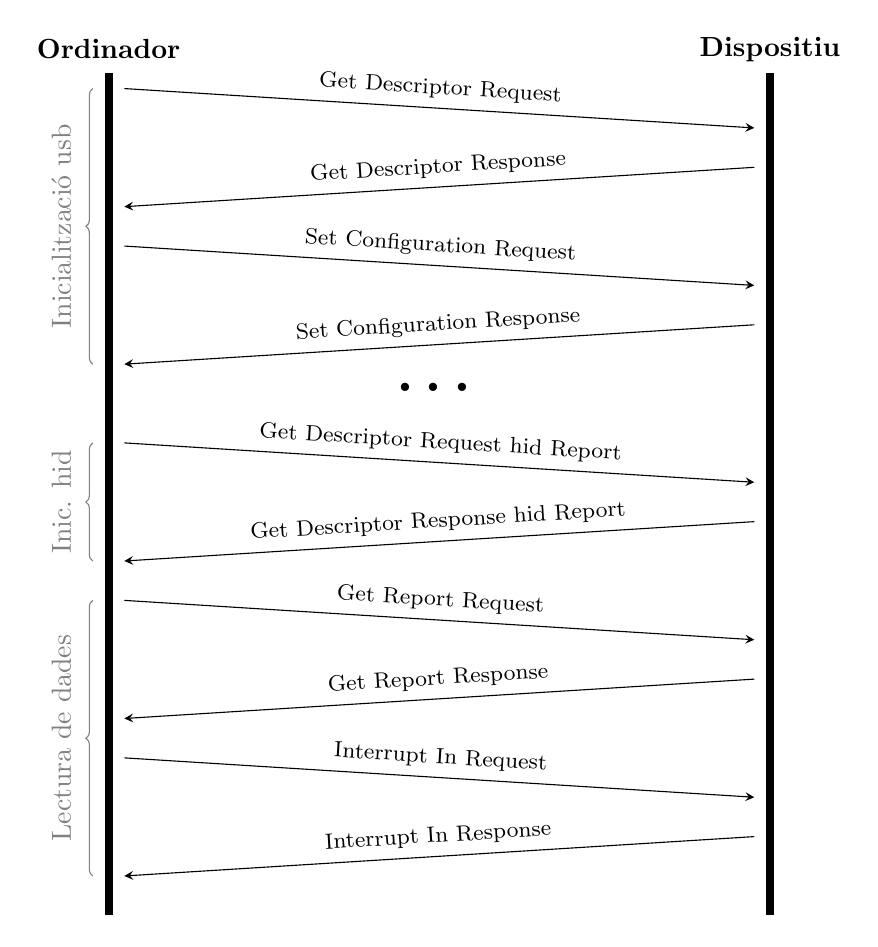
\begin{tikzpicture}[>=stealth]

            \node at (-0.2,0) {\textbf{Ordinador}};
            \node at (8.2,0) {\textbf{Dispositiu}};

            \draw[-] [line width=1mm, black] (-0.2,-0.3) -- (-0.2,-11);
            \draw[-] [line width=1mm, black] (8.2,-0.3) -- (8.2,-11);
        
            % Arrows for packets
            \draw[->] (0,-0.5) -- (8,-1) node[midway, above, sloped] {\footnotesize \acro{Get Descriptor} Request};
            \draw[->] (8,-1.5) -- (0,-2) node[midway, above, sloped] {\footnotesize \acro{Get Descriptor} Response};
            \draw[->] (0,-2.5) -- (8,-3) node[midway, above, sloped] {\footnotesize \acro{Set Configuration} Request};
            \draw[->] (8,-3.5) -- (0,-4) node[midway, above, sloped] {\footnotesize \acro{Set Configuration} Response};
        
            \node at (4, -4.3) {\huge \textbf{\dots}};

            \draw[->] (0,-5) -- (8,-5.5) node[midway, above, sloped] {\footnotesize \acro{Get Descriptor} Request \acro{hid} Report};
            \draw[->] (8,-6) -- (0,-6.5) node[midway, above, sloped] {\footnotesize \acro{Get Descriptor} Response \acro{hid} Report};

            \draw[->] (0,-7) -- (8,-7.5) node[midway, above, sloped] {\footnotesize \acro{Get Report} Request};
            \draw[->] (8,-8) -- (0,-8.5) node[midway, above, sloped] {\footnotesize \acro{Get Report} Response};
            \draw[->] (0,-9) -- (8,-9.5) node[midway, above, sloped] {\footnotesize \acro{Interrupt In} Request};
            \draw[->] (8,-10) -- (0,-10.5) node[midway, above, sloped] {\footnotesize \acro{Interrupt In} Response};

            % Braces
            \draw [decorate, decoration={brace, mirror}, gray] (-0.4,-0.5) -- (-0.4,-4);
            \draw [decorate, decoration={brace, mirror}, gray] (-0.4,-5) -- (-0.4,-6.5);
            \draw [decorate, decoration={brace, mirror}, gray] (-0.4,-7) -- (-0.4,-10.5);

            \node [gray] at (-0.8, -2.25) {\rotatebox{90}{Inicialització \acro{usb}}};
            \node [gray] at (-0.8, -5.75) {\rotatebox{90}{Inic. \acro{hid}}};
            \node [gray] at (-0.8, -8.75) {\rotatebox{90}{Lectura de dades}};

        \end{tikzpicture}
    %\end{adjustbox}

    \caption{Exemple simplificat d'intercanvi de paquets entre un ordinador i un dispositiu \acro{hid}.}
    \label{fig:hid-packets}
\end{figure}
